\section{Search}
The Zimbra Drive search feature appears upon selecting the drive item in the dropdown search menu or changing to the drive view.
The Zimbra Drive icon in the search toolbar means that the following search will be performed to the user own drive.
\begin{figure}[htbp,!h] 
\centering 
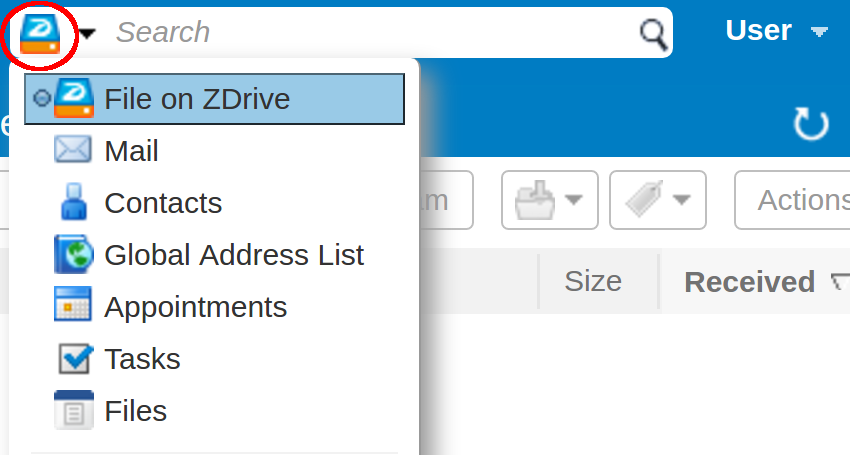
\includegraphics[scale=0.25]{src/images/ZD-searchMenu.png} 
\caption{Search Menu Item} 
\label{==fig:searchMenu==}
\end{figure}

The search feature has a 'string filter' and a 'location command'. 
Every search is threated as not case sensitive. \\
The string filter locates the files and the folders which names contains the string given (not case sensitive).
E.g: the results of the filter 'mp' can be "EXAMPLE.txt" and "Improvement.pdf".\\

The location command is in the following expression:
\begin{verbatim}
in:"/Documents"
\end{verbatim}
If the search is performed with just a 'location command', the results will be only the contents of the specific folder.\\

Any different search combination of multiple 'string filter' and a possible 'location command' returns 
the files and the folders matched in a recursive search.

\begin{warning}
    Multiple location commands are compared with an AND operator that makes them useless. Don't use them.
\end{warning}
